\chapter{PLC State Machine Flowcharts}
\label{ch:PLC-flowcharts}


\section{Communications State Machine}
\label{sec:PLC-flowcharts-comms}

	\begin{center}
		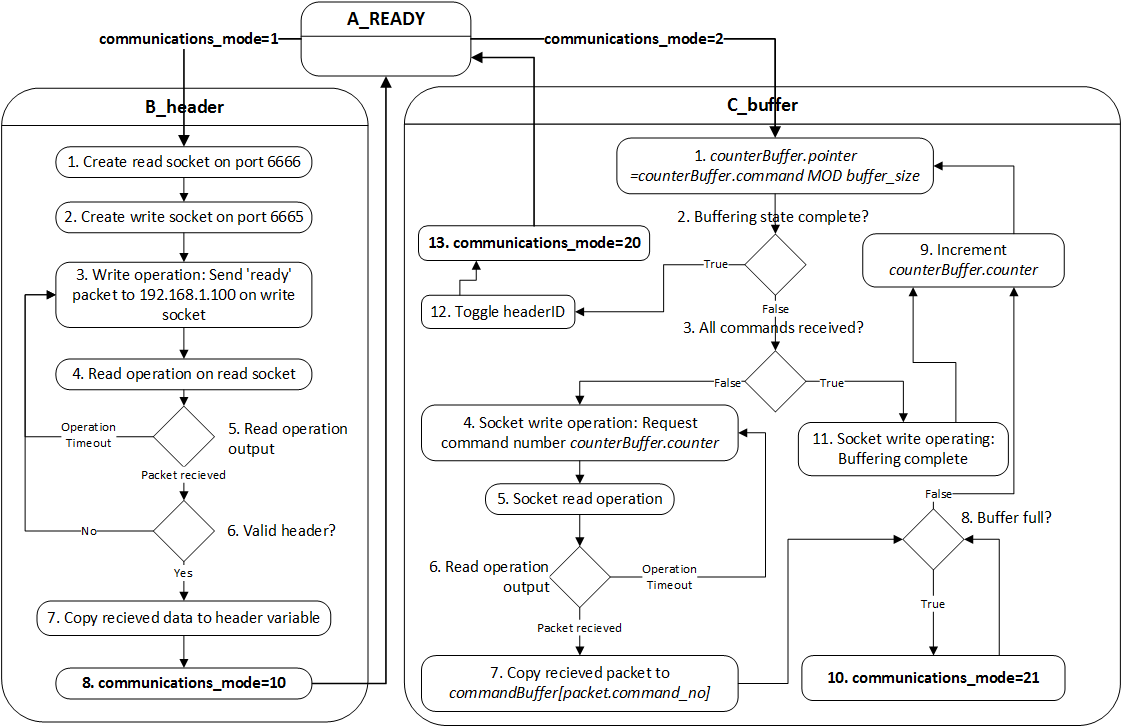
\includegraphics[width=\textwidth]{figures/cncMachine/communications}
		\captionof{figure}{Communications program: States and State Actions}
		\label{fig:communicationsStates}
	\end{center}

\section{motorControl State Machine}
\label{sec:PLC-flowcharts-motor}
	\begin{center}
		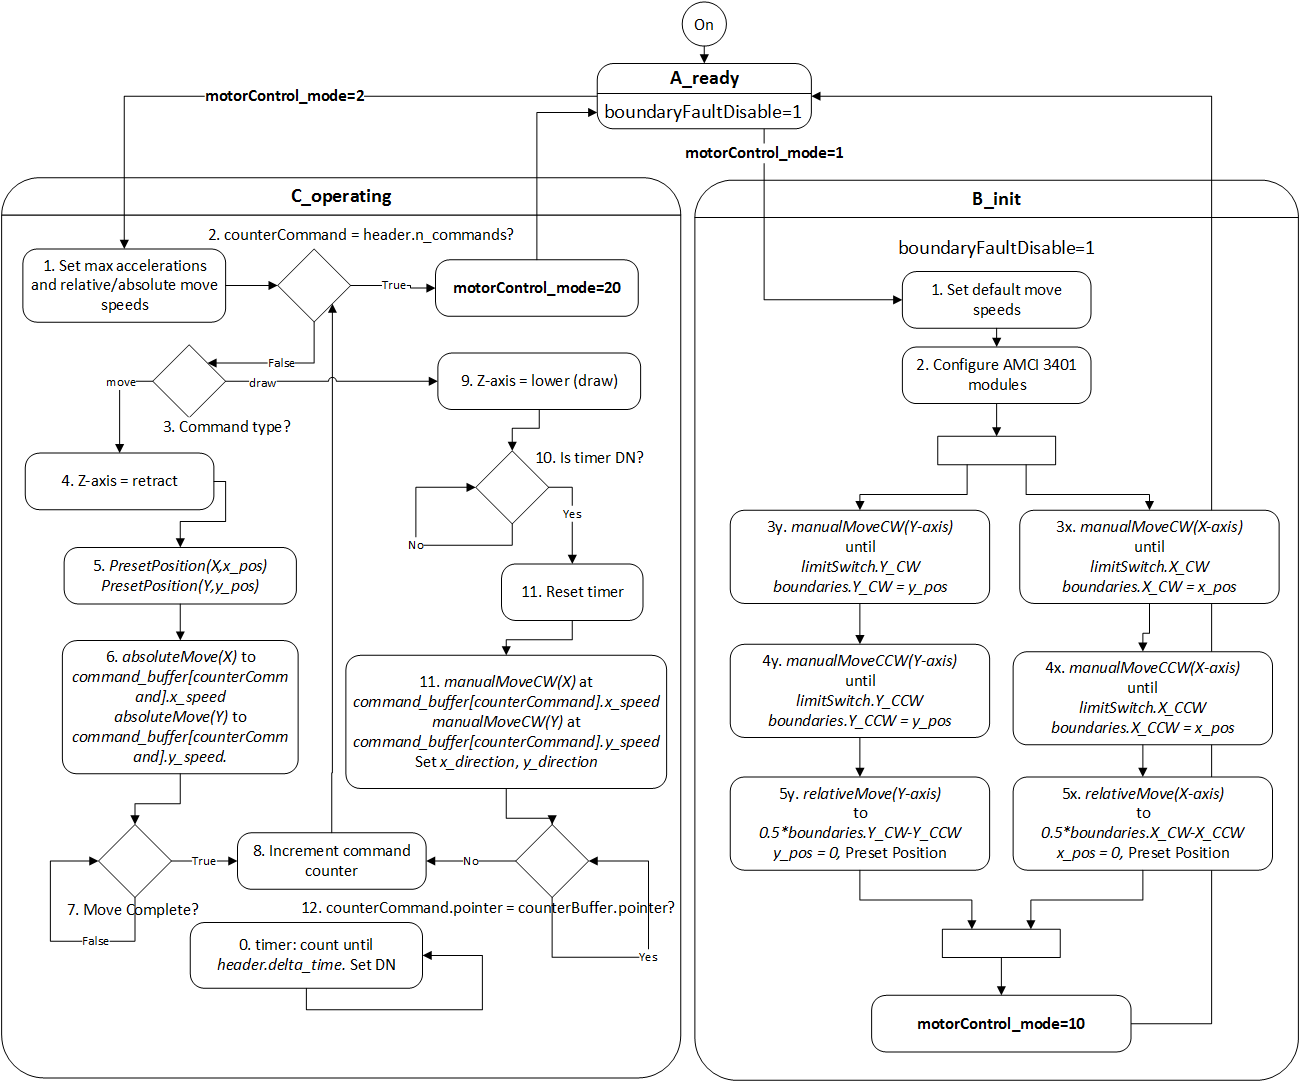
\includegraphics[width=\textwidth]{figures/cncMachine/motorControl}
		\captionof{figure}{motorControl Program: States and State Actions}
		\label{fig:motorControlStates}
	\end{center}

	\subsubsection{Introduction to the AMCI 3401 Stepper Module}
			The main purpose of the motorControl program is to communicate with the two AMCI 3401 Stepper Motor Modules. Their primary role is to send two types of control signals to the stepper motor modules:\\
			\begin{description}
				\item[Step Output] \hfill \\
					A $5V$ square pulse output, with each rising edge signifying a single step of the motor.
				\item[Direction Output] \hfill \\
					A $5V$ boolean output that defines which direction the stepper motors should turn.
			\end{description}
			The modules takes its input by asynchronously monitoring a 16-byte command word on the PLC and mirror it internally. All commands given by the motorControl program involving modifying this command word. \\
			In addition, the module monitors its relative position and operating state by providing a 16-byte status word.\\
			The modules feature a broad range of commands, but the those used by the DoodleBot system are:
			\begin{description}
				\item[Absolute Move] \hfill \\
					Given a position in space (relative to the preset origin position), the AMCI module creates the appropriate velocity profile to get there (within the acceleration/deceleration/top speed parameter limits).
				\item[Relative Move] \hfill \\
					Given a distance to travel (from the current position), the AMCI module creates the appropriate velocity profile to get there (within the acceleration/deceleration/top speed parameter limits).
				\item[Manual Move] \hfill \\
					Manual type moves are actually classified as two separate commands defining the direction of the move  - manual move clockwise, and manual move counterclockwise. These moves accelerate to the programmed speed at the acceleration rate and travel until stopped. While moving in this state, the programmed speed can be changed without having to stop and restart.
				\item[Immediate Stop] \hfill \\
					An immediate stop command stops all current motion.
				\item[Preset Current Position] \hfill \\
					Sets the internal position memory of the module to a position defined in the command word.
			\end{description}

\subsection{Position and Direction Control}
\label{sec:PLC-flowcharts-pos}

	\begin{figure}[htbp!]
		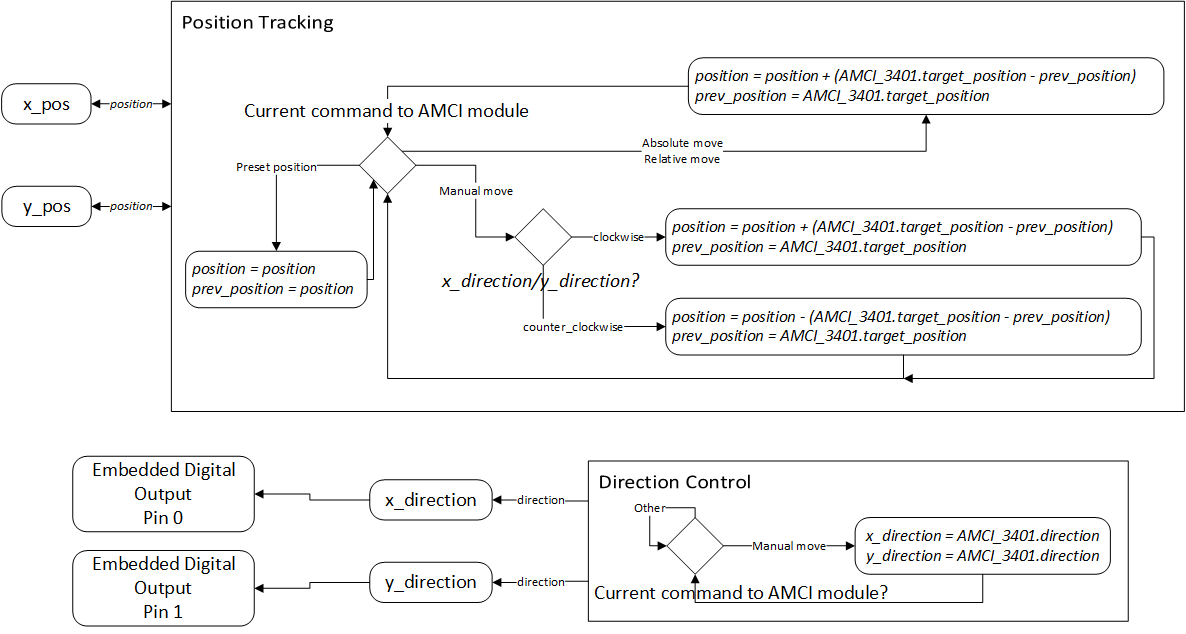
\includegraphics[width=\textwidth]{figures/cncMachine/position_direction}
		\caption{The two routines for managing direction and position}
		\label{fig:Direction and Positional Tracking}
	\end{figure}
	
				\begin{description}
					\item[Absolute Move, Relative Move] \hfill \\
						Relative Moves are treated by the rest of the code as usual. Absolute Moves must be preceded by a Preset Current Position command with the position set to x\_pos and y\_pos. <blah> function monitors the directional state of the AMCI 3401 modules and mirrors this onto the direction output pins. <gah> function measures the change in position since last scan and adds this to x\_pos and y\_pos.
					\item[Manual Move] \hfill \\
						All manual moves, whether clockwise or anticlockwise, are sent to the AMCI 3401 modules as Manual Move Clockwise at the correct speed. The x\_direction and y\_direction bits need to be explicitly set with each Manual Move command to operate in the required direction. Since the AMCI 3401 module thinks it is always moving clockwise (even when it's not), it's internal position state is no longer correct. Function <gah> measures the change in position since last scan and depending on the direction of movement, adds or subtracts this value to x\_pos and y\_pos.
					\item[Preset Current Position] \hfill \\
						Change the value of x\_pos and y\_pos to mirror the position state in the AMCI 3401 controller.
				\end{description}